%!TEX program = xelatex
\documentclass[cn,geye,cyan,normal,14pt]{elegantnote}
\usepackage{texnames}%输出\TeX家族标志符
\title{Jabref和Zotero使用笔记}
\author{\href{mailto:zalois@126.com}{zalois@126.com}}
\institute{欢迎自由修改分享交流}
\date{\zhtoday}
%\version{0.00}
\setCJKmainfont[AutoFakeBold = {2.17}]{FZLanTingHeiPro_GB18030}%设置中文主字体为方正兰亭黑Pro字体
%\setCJKmainfont[AutoFakeBold = {2.17}]{Adobe Song Std L}%设置中文主字体为Adobe 宋体
\newcommand{\hei}{\CJKfontspec{Adobe Heiti Std R}}%Adobe 黑体
\newcommand{\kai}{\CJKfontspec{Adobe Kaiti Std R}}%Adobe 楷体
\newcommand{\fs}{\CJKfontspec{Adobe Fangsong Std R}}%Adobe 仿宋
\newcommand{\lei}{\CJKfontspec[ExternalLocation=/media/sdb6/TeX/fonts/cnFonts/钢笔字/]{方正徐静蕾简体.ttf}}%徐静蕾字体
\begin{document}
\maketitle
\section{摘要}
Jabref和Zotero都可以用来管理文献,提高嗑盐效率。本文主要记录的是添加文献条目到Jabref的文献库中的方法,以及如何在源文件中比较方便的一键引用参考文献条目。
本文没有介绍具体参考文献列表格式及其制作;也没有介绍源文件中引用参考文献的样式的个性化修改。\footnote{本文适用人群:刚入门嗑盐,和作者一样,不想手工一条一条排序的人。%
\\不适用人群:通过手工一条一条排序调节嗑盐生活,并以此为乐的神人。}
\section{关键词}
参考文献,一键引用,文本编辑器
\section{前期准备}
\begin{itemize}
	\item 您的机器上最好有\href{https://www.tug.org/texlive/}{\TeX live},或者类似的\TeX 程序。
	\item 文本编辑器最好是\href{https://github.com/texstudio-org/texstudio/releases}{\TeX studio},如果您是用\href{https://github.com/vim/vim/releases}{Vim}或者\href{https://ftp.gnu.org/gnu/emacs/}{Emacs}的人,您可以不用浪费时间阅读本文。
	\item 您的机器上有\href{https://github.com/JabRef/jabref/releases}{Jabref}或\href{https://github.com/zotero/zotero/releases}{Zotero}程序(最好两者都有)。Jabref目前最新的稳定版是4.3.1(Jabref是用JAVA语言开发的,需要JAVA运行环境,可以安装jre8),您也可以用 5.0 的开发版(这个集成了最新的JAVA环境,做到了开箱即用),本人更喜欢后者。\footnote{Jabref 4.3.1 下载链接:\url{https://github.com/JabRef/jabref/releases/tag/v4.3.1},\\
		Jabref 5.0 开发版下载链接:\url{https://github.com/JabRef/jabref/releases/tag/v5.0-beta},\\
		jre 8 下载链接:\url{https://www.oracle.com/technetwork/java/javase/downloads/jre8-downloads-2133155.html},\\
		Zotero 5.0.80 下载链接:\url{https://github.com/zotero/zotero/releases/tag/5.0.80},\\
		您也可以安装平常用的多的浏览器对应的插件,下载链接:\url{https://www.zotero.org/download/}。}
\end{itemize}
\section{重点一:制作bib文献数据库}
.bib文件实际上是一个格式化的文本文件。里面一条一条记录形如:
\begin{lstlisting}
@Article{Douglas1966,
  author    = {R. G. Douglas},
  title     = {On majorization, factorization, and range inclusion of operators on Hilbert space},
  journal   = {Proceedings of the American Mathematical Society},
  year      = {1966},
  volume    = {17},
  number    = {2},
  pages     = {413--413},
  month     = {feb},
  doi       = {10.1090/s0002-9939-1966-0203464-1},
  publisher = {American Mathematical Society ({AMS})},
}
\end{lstlisting}
对于Jabref,添加.bib文献数据库的条目方法很多,手工一条条直接添加也可以。但是我们一般情况不用这么麻烦的,这里着重介绍两种添加参考文献条目的方法\footnote{这两种方法都需要在联网的情况下才能完成。}:
\clearpage
	\begin{itemize}
		\item 第一类,对于有明确序号的如MathSciNet的MR,DOI,ArXiv,ISBN之类的文献,可以直接选择这里,
			\begin{center}
				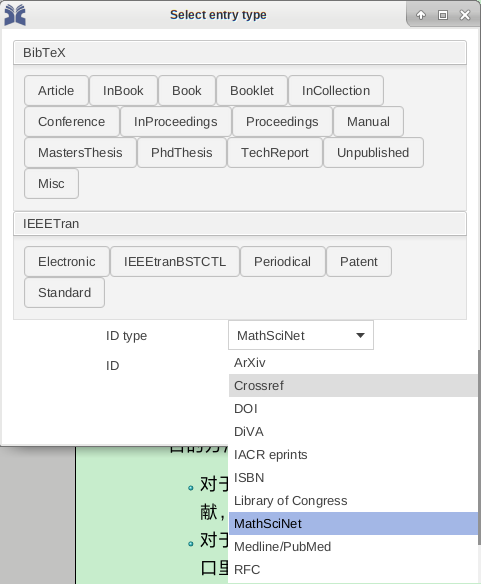
\includegraphics[width=0.618\textwidth]{pictures_01.png}
			\end{center}
			再点击
			\begin{center}
				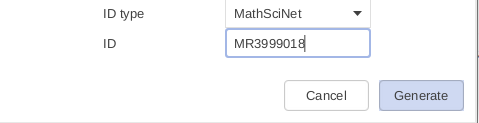
\includegraphics[width=0.618\textwidth]{pictures_02.png}
			\end{center}
			这样,就加入了,最终效果如图:
			\begin{center}
			
\includegraphics[width=0.618\textwidth]{pictures_03.png}
			\end{center}
		\item 第二类,手工添加引用信息到.bib文件。对于百度学术,选择引用,
			\begin{center}
			
\includegraphics[width=0.618\textwidth]{pictures_04.png}
			\end{center}
			选择 \BibTeX,
			\begin{center}
			
\includegraphics[width=0.618\textwidth]{pictures_05.png}
			\end{center}
			弹出来的窗口里全选复制
			\begin{center}
			
\includegraphics[width=0.618\textwidth]{pictures_06.png}
			\end{center}
			再用文本编辑器打开.bib文件,粘贴到最后位置即可,注意保存一下。\\
对于谷歌学术,选择逗号,
			\begin{center}
			
\includegraphics[width=0.618\textwidth]{pictures_07.png}
			\end{center}
			其余操作类似,最终是这样效果:
			\begin{center}
			
\includegraphics[width=0.618\textwidth]{pictures_08.png}
			\end{center}
	\end{itemize}
	\begin{note}
在Windows系统下,如果用文本编辑器打开.tex或者.bib文件是乱码,这是由于Windows创建的文本文件默认编码是ANSI,可以用“记事本”打开,“另存为”,编码格式选“utf8”,重新保存成utf8编码的文件即可。这样的操作也可以反过来,utf8编码的可以转成ANSI,适用于用传统编码的文本编辑器(如WinEdt)。\\
对于Zotero,强大在可以进行文献管理,可以从有标志的pdf文件里自动提取信息生成文献列表信息。对中文期刊支持很好,支持大陆版的DOI等,也可以导出生成.bib文件。
	\end{note}
\section{重点二:在\TeX 源文件中使用生成的参考文献列表}
\textcolor{red}{需要注意的是.bib文件和.tex文件最好放在同一文件夹下。如果不是,需要在源文件中指明具体的路径和文件名,不需要扩展名.bib。}
\begin{itemize}
	\item 一般是在\TeX 源文件末尾加入这样两行:
		\begin{lstlisting}
			\bibliographystyle{plain}
			\bibliography{bib文件名1,bib文件名2,...}
		\end{lstlisting}
			\begin{note}
				此处plain是参考文献列表格式,我国出版机构文后参考文献著录规则大部分采用的是国标\href{http://www.sac.gov.cn/SACSearch/outlinetemplet/gjbzcx.jsp}{GB/T 7714}\cite{gbt7714_2015},最新的是\href{http://www.scal.edu.cn/dxtsgxb/201906120155}{2015}年修订的\footnote{本文模板采用的文后参考文献著录规则就是GB/T 7714}。具体的格式要看您投稿的机构,一般都会提供相应格式的.bst配置文件。当然生猛的您可以自己手工修改相应的.bst文件,调整格式,见\href{https://blog.csdn.net/chikily_yongfeng/article/details/86553359}{\LaTeX 自定义参考文献格式(配置 bst)}\cite{noauthor_latex_nodate}。
			\end{note}
如果希望bib文件中所有文献都列出来,在这两句话前面再加一句话:
		\begin{lstlisting}
			\nocite{*}
		\end{lstlisting}
否则,只有前面引用的才会出现在生成的参考文献列表里。
	\item 插入引用标志到文中具体位置,按如下“三步走”:
		\begin{itemize}
			\item 第一步,先在文本编辑器比如\TeX studio中,打开要编辑的.tex文件,把光标定位在要插入引用文献标志的位置;
			\begin{center}
			
\includegraphics[width=0.618\textwidth]{pictures_12.png}
			\end{center}
		\item 第二步,在Jabref中打开.bib文件,选择要插入的参考文献条目,多选按住Ctrl键。
			\begin{center}
			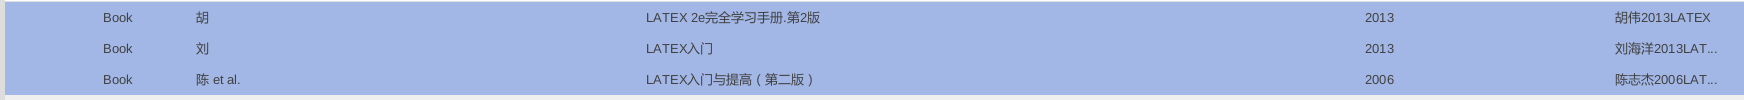
\includegraphics[width=0.618\textwidth]{pictures_13.png}
			\end{center}
		\item 第三步,点击工具条中的图标
\includegraphics{pictures_11.png},或者按Ctrl+L键。
			\begin{center}
			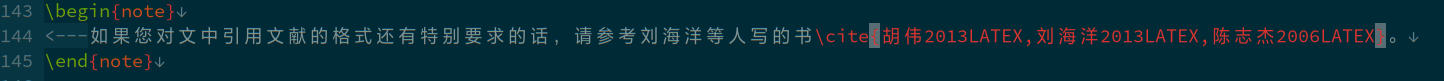
\includegraphics[width=0.618\textwidth]{pictures_14.png}
			\end{center}
		\end{itemize}
\end{itemize}
您会发现引用文献标志已经加到相应位置了,是不是很方便?有没有很惊喜?\\
如果您的Jabref工具栏中没有
\includegraphics{pictures_11.png},您需要在菜单栏选\\
``Options''$\to$``Preferences''$\to$``External programs'',\\
再从下拉菜单中选择您所用的文本编辑器,目前Jabref支持的编辑器有 \href{https://ftp.gnu.org/gnu/emacs/}{Emacs}, \href{https://www.lyx.org/}{Lyx}/\href{https://kile.sourceforge.io/}{Kile},\href{https://www.xm1math.net/texmaker/}{\TeX maker},\href{https://github.com/texstudio-org/texstudio/releases}{\TeX studio},\href{https://github.com/vim/vim/releases}{Vim},\href{http://www.winedt.com/}{WinEdt} 六种。
			\begin{center}
			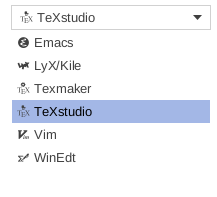
\includegraphics[width=0.618\textwidth]{pictures_10.png}
			\end{center}
\begin{note}
	如果手工引用参考文献,直接复制对应文献条目的具体Bibtexkey值,
			\begin{center}
			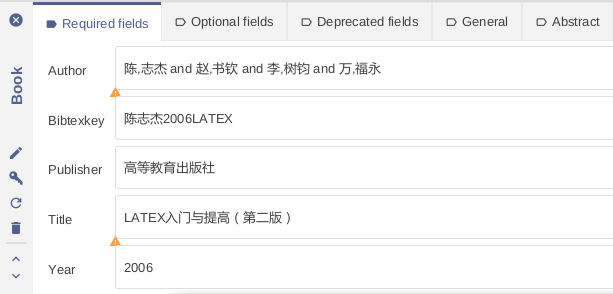
\includegraphics[width=0.618\textwidth]{pictures_15.png}
			\end{center}
			或者.bib文件中这个位置的字符串,下图中对应的红色部分的字符串:
			\begin{center}
			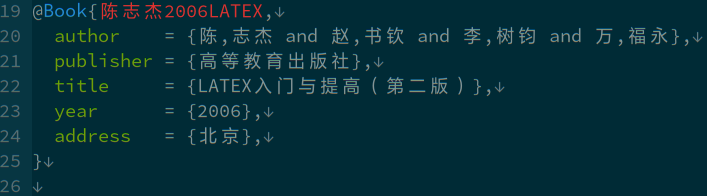
\includegraphics[width=0.618\textwidth]{pictures_16.png}
			\end{center}
	然后在源文件对应位置用如下命令即可:
	\begin{lstlisting}
	\cite{具体Bibtexkey值}
	\end{lstlisting}
\end{note}
\begin{note}
	如果您对文中引用文献的格式还有特别要求的话,请参考刘海洋等人写的书\cite{胡伟2013LATEX,刘海洋2013LATEX,陈志杰2006LATEX}。
\end{note}
\section{编译}
如果是\TeX studio编辑器的话,直接点
\includegraphics{pictures_17.png}(按F5效果同)或者
\includegraphics{pictures_18.png}(按F6效果同)就可以了。
如果您用的是别的编辑器(比如Vim,Emacs,WinEdit之类的),您需要执行如下四步\cite[第 380 页]{胡伟2013LATEX}:
\begin{itemize}
	\item 第一步:先编译.tex源文件一次,
	\item 第二步:用\BibTeX 编译.bib文件,参考命令:
		\begin{lstlisting}
		bibtex   具体bib文件名
		\end{lstlisting}
	\item 第三、四步:编译.tex文件\textcolor{red}{两}次,就可以正确生成引用位置了(否则引用位置有可能会出现问号,形如[?])。
\end{itemize}
\section{利益无关声明}
本文涉及到的程序,除了WinEdt是商业软件外,其余如\TeX 系统,Jabref和Zotero文献管理器,Vim,Emacs,\TeX studio等文本编辑器都是开源软件。本文也是以开源协议发布的,欢迎大家在开源协议下自由修改分享。本文链接:\url{https://github.com/zalois/note4JabrefandZotero}
\section{致谢}
感谢创建\TeX 的Donald Ervin Knuth先生,感谢Jabref和Zotero的贡献者们。
本文档套用的模板下载自\href{https://github.com/ElegantLaTeX/ElegantNote}{https://github.com/Elegant\LaTeX/ElegantNote},感谢模板作者邓东升。\footnote{插播一个小广告:本文档系统环境:\href{https://mirrors.slackware.com/slackware/slackware64-current/}{Slackware64-Current} + \href{https://www.tug.org/texlive/}{\TeX live 2019} + \href{https://www.vim.org/}{Vim 8.2.90}}
%\nocite{*}
%\bibliographystyle{plain}
\bibliography{Jabref和Zotero使用笔记}
\end{document}
